%
% LaTeX report template 
%

% This is a comment: in LaTeX everything that in a line comes
% after a "%" symbol is treated as comment

\documentclass[11pt, a4paper]{article}
\usepackage{graphicx}
\usepackage{amsmath}
\usepackage{listings}


\title{Assignment No 8} % Title

\author{Prasanna Bartakke EE19B106} % Author name

\date{\today} % Date for the report
\begin{document}		
		
\maketitle % Insert the title, author and date
\section{Aim}
%Create new section;it is autonumbered
The aim of this assignment is to examine the DFT of various functions using the fft library in numpy.
\section{Sinusoid}
In this part we study the spectrum of $sin(5t)$. As expected, we get 2 peaks at +5 and -5 with height 0.5. The phase at the peaks are $\pi / 2 $ and $-\pi / 2$.
\begin{equation}
y = sin(5t) = 0.5(\frac{e^{5t}}{j}-\frac{e^{-5t}}{j})
\end{equation}
\begin{figure}[!tbh]
   	\centering
   	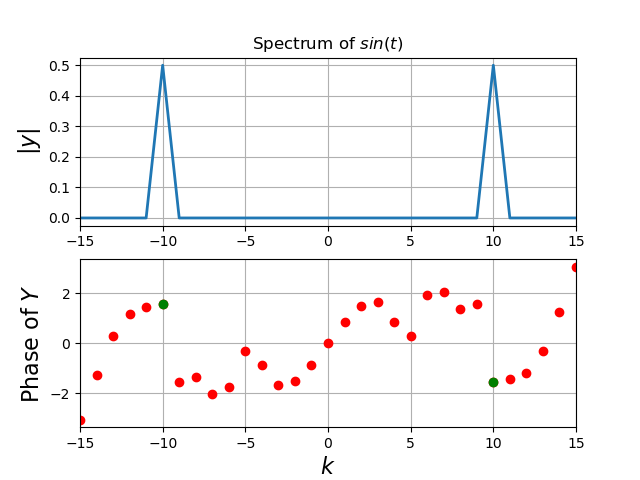
\includegraphics[scale=0.5]{fig0.png}  % Mention the image name within the curly braces. Image should be in the same folder as the tex file. 
   	\caption{DFT of $sin(5t)$}
   	\label{fig:sample}
   \end{figure} 
\section{Amplitude Modulated Signal}
The amplitude modulated signal is,
\begin{equation}
f(t) = (1+0.1\cos(t))\cos(10t)    
\end{equation}

By using a larger range and higher number of samples, we can see the three peaks clearly. At all three peaks the phase is zero.
\begin{figure}[!tbh]
   	\centering
   	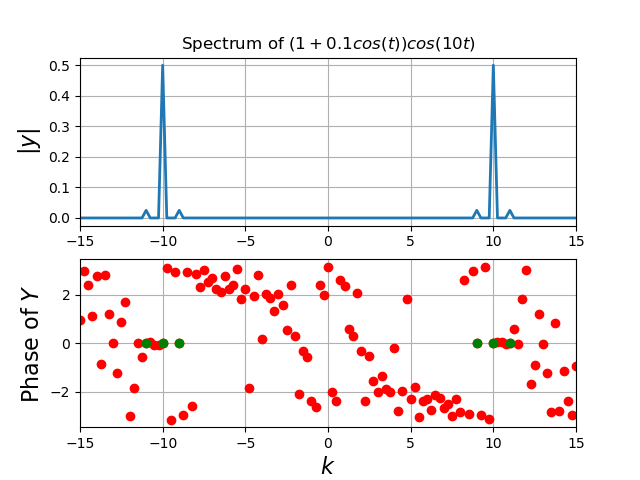
\includegraphics[scale=0.5]{fig1.png}  % Mention the image name within the curly braces. Image should be in the same folder as the tex file. 
   	\caption{DFT of am signal}
   	\label{fig:sample}
   \end{figure} 
\section{Spectrum of $sin^3(t)$ and $cos^3(t)$}
The signals can be represented as follows:
\begin{equation}
\sin^3(t) = \frac{3}{4}\sin(t) - \frac{1}{4}\sin(3t)
\end{equation}
\begin{equation}
\cos^3(t) = \frac{3}{4}\cos(t) + \frac{1}{4}\cos(3t)
\end{equation}
\begin{figure}[!tbh]
   	\centering
   	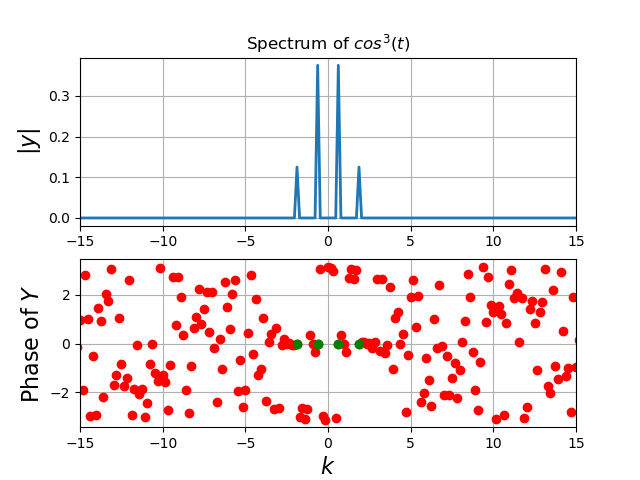
\includegraphics[scale=0.5]{fig2.png}  % Mention the image name within the curly braces. Image should be in the same folder as the tex file. 
   	\caption{DFT of $cos^3(t)$}
   	\label{fig:sample}
   \end{figure} 
 \begin{figure}[!tbh]
   	\centering
   	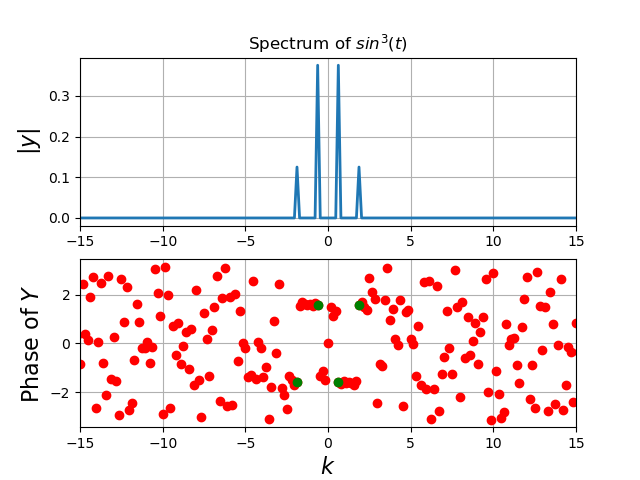
\includegraphics[scale=0.5]{fig3.png}  % Mention the image name within the curly braces. Image should be in the same folder as the tex file. 
   	\caption{DFT of $sin^3(t)$}
   	\label{fig:sample}
   \end{figure} 
Thus there will be 4 impulses in the frequency spectrum. Following are the spectrums obtained.

\newpage
\section{Frequency Modulation}
Consider the frequency modulated signal, $\cos(20t + 5\cos(t))$
\begin{figure}[!tbh]
   	\centering
   	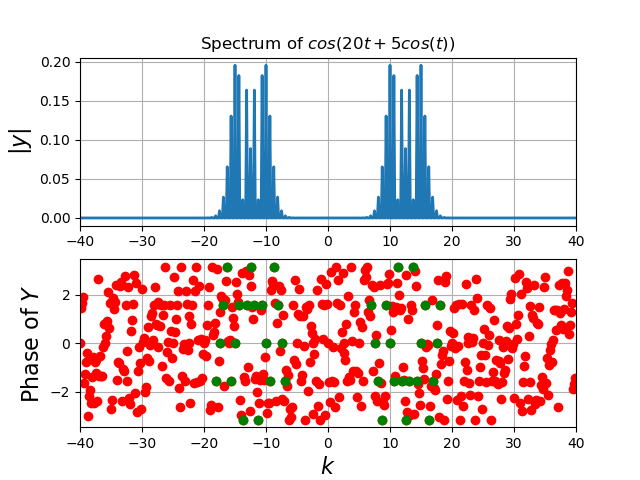
\includegraphics[scale=0.5]{fig4.png}  % Mention the image name within the curly braces. Image should be in the same folder as the tex file. 
   	\caption{DFT of fm signal}
   	\label{fig:sample}
   \end{figure} 
   
   
\newpage
\section{Gaussian}
The Gaussian function $f(x) = e^{-x^2/2}$ is not band limited as the frequency spectrum has non zero values even for large frequencies.
The value of error varies with different time ranges and the sampling rate. For sampling rate = 512 and time range = $8\pi$ s, the error is found to be around $10^{-15}$.
As the sampling rate increases, the peak sharpens. Also, it broadens for greater time ranges.
\begin{figure}[!tbh]
   	\centering
   	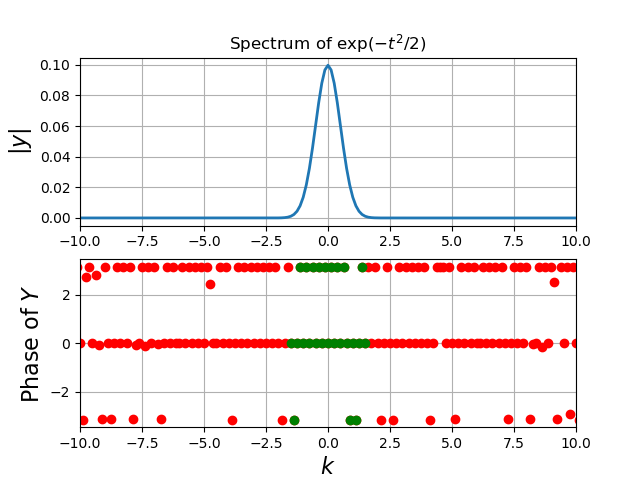
\includegraphics[scale=0.5]{fig6.png}  % Mention the image name within the curly braces. Image should be in the same folder as the tex file. 
   	\caption{DFT of gaussian for time range = $8\pi$ and sampling rate = 512}
   	\label{fig:sample}
   \end{figure} 


\begin{figure}[!tbh]
   	\centering
   	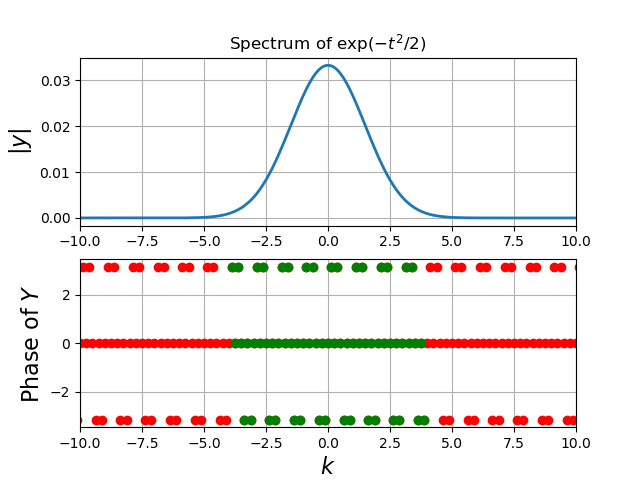
\includegraphics[scale=0.5]{fig7.png}  % Mention the image name within the curly braces. Image should be in the same folder as the tex file. 
   	\caption{DFT of gaussian for time range = $12\pi$}
   	\label{fig:sample}
   \end{figure}
   
\begin{figure}[!tbh]
   	\centering
   	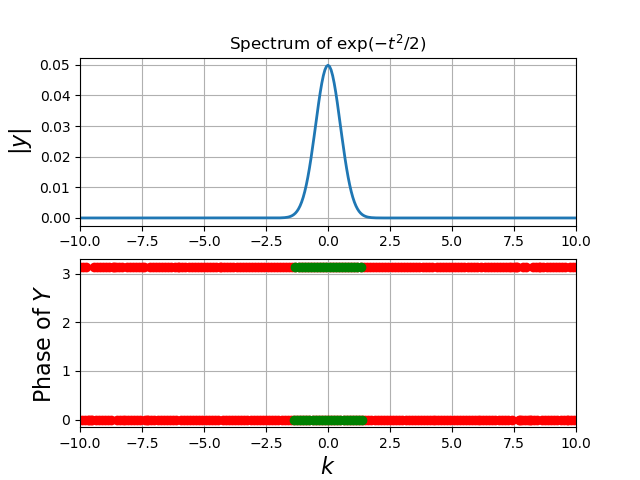
\includegraphics[scale=0.5]{fig9.png}  % Mention the image name within the curly braces. Image should be in the same folder as the tex file. 
   	\caption{DFT of gaussian for sampling rate = 1024}
   	\label{fig:sample}
   \end{figure} 
 
 \begin{figure}[!tbh]
   	\centering
   	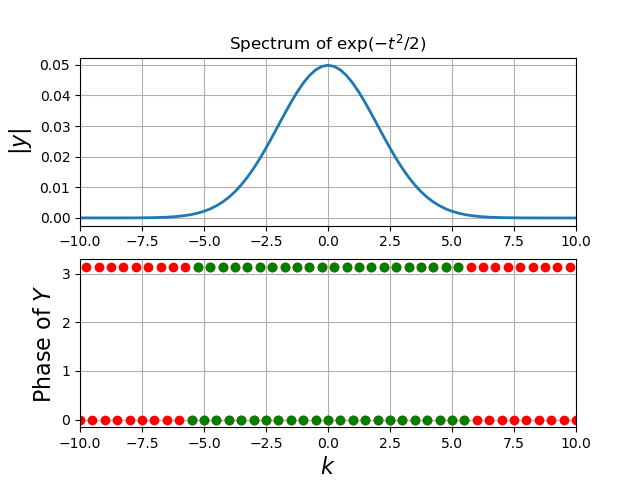
\includegraphics[scale=0.5]{fig8.png}  % Mention the image name within the curly braces. Image should be in the same folder as the tex file. 
   	\caption{DFT of gaussian for sampling rate = 256}
   	\label{fig:sample}
   \end{figure} 

\end{document}



 